
\chapter{Evaluation Of Integrals}

\section{Discussion Of The Integrands}

\subsection{Finite Element Integrals}

In a basic finite element method the only integrals that need to be evaluated are those giving the residuals. After discretisation these take the form of sums of shape functions multiplied by test functions (and/or derivatives of either). Hence if the shape and test functions are chosen to be polynomials, as is usually the case, then the integrals can easily be evaluated using e.g. a Gauss-Legendre quadrature scheme of appropriate order designed for the element geometry \cite{??ds: Gauss-Legendre schemes for arbitrary geometry, Milan gave Mousavi2010 but it is more about polygons with large numbers of sides not 3D ones}.

For example we typically use shape and test functions which are both polynomials of degree $a$. In this case a Gauss-Legendre quadrature scheme with $a$ points  will be able to exactly and efficiently evaluate the required integrals.

\subsection{Hybrid Boundary Element Integrals}

Some of the integrals to be evaluated in boundary element methods contain singular or near singular terms. As such they are much more difficult to evaluate than the integrals encountered in the finite element method. Hence the rest of this section will focus on these integrals.

In $d$ dimensions for target node $i$ and source node $j$ (see \cref{sec:hybr-finit-elem}, equation~\cref{eq:19}) the non-constant part of the boundary element integral is:
\begin{equation}
  \label{eq:7}
   I_{\ibasis\ibasisb} = \int_{\boundd_\ibasis} \psi_\ibasis(\yv) \frac{\nv \cdot \ruv_{\ibasis,\ibasisb}}{| \xv_\ibasisb - \yv| ^{d-1}} d\yv.
\end{equation}
There are three key parts to the integrand: firstly the basis function $\psi(\yv)$ which is a simple polynomial and poses no problems. Secondly the singular part $ \frac{1}{|\xv_\ibasisb - \yv| ^{d-1}}$ which is difficult to integrate when the source node $\xv_\ibasisb$ is close to the element we are integrating over. Finally there is the dot product of the unit normal and the unit vector in the direction of the singularity. For flat elements this is zero in the singular case. For curved elements my numerical experiments show that it approaches zero at approximately the same rate as the singular part approaches infinity - hence it reduces the singularity by one order.

??ds - really need to make this more rigorous. This also introduces a dependence on the geometry of the element for all cases.

So for three-dimensional problems we still have a weakly singular integral to deal with.

??ds not done yet... probably goes in another section... We deal with this using a change of variables as described by Telles \cite{Telles1987}.

??ds or not - according to other references Telles does not remove the singularity?

Another point worth noting is that O(N$_b$) similar integrals are calculated over each element.
Hence it should be possible to reuse the calculations of shape function, interpolated position and normal unit vector between integrals which use the same order of quadrature.

\section{Standard Quadrature Schemes}

Numerical quadrature schemes attempt to approximate integrals using a summation of the form
\[ \int_a^b f(x) \, dx = \sum_{i=0}^N w_i \, f(x_i). \]

The points $x_i \in \real^d$ are known as the \emph{knots}\footnote{The evaluation points are more commonly known as the nodes but we already use ``nodes'' to mean something else in a finite element context.} of the scheme and the numbers $w_i \in \real$ are known as the \emph{weights}.
Alternatively a weight function can be introduced to optimise the scheme for integrands of a specific form, if $f(x) = W(x) g(\xv)$ then
\begin{equation}
  \label{eq:9}
  \int_a^b W(x) g(x) \, dx = \sum_{i=0}^N w_i' \, g(x_i).
\end{equation}

The \emph{degree} of a quadrature scheme is the maximum degree of polynomial that can be integrated exactly by the scheme (for all other functions the quadrature is only an approximation).
This is often considered to be a good measure of the accuracy of the scheme, but may not be appropriate in some cases \cite{Trefethen2008}.
The highest degree possible is $2n + 1$ where $n + 1$ is the number of points used by the scheme ??ds-citation.

A quadrature scheme is \emph{progressive} (or \emph{nested}) if higher order schemes can reuse knots from lower order schemes.

Some commonly used quadrature schemes are:

\subsection{Newton-Cotes}
\begin{itemize}
\item The most basic quadrature method, also known as the trapezoidal rule.
\item Degree is $n$.
\item Knots are uniformly spaced.
\item Weights are all $1/n + 1$.
\item Progressive
\end{itemize}

\subsection{Gaussian Quadratures}
\begin{itemize}
\item Optimal degree: $2n +1$.
\item The most commonly used quadrature scheme.
\item The knots, $x_i$, are the roots of the $(n+1)$-th orthogonal polynomial on $[a,b]$ with the weight function $W(x)$. $W(x) = 1$ gives Gauss-Legendre quadrature (the orthogonal polynomials are the Legendre polynomials).
\item Not progressive.
\item The Gauss-Kronrod or Patterson rules be used to create a semi-progressive scheme.
\end{itemize}

\subsection{Clenshaw-Curtis}
\begin{itemize}
\item Degree $n$.
\item The degree may not actually reflect the accuracy of the scheme. It is only significantly outperformed by Gauss-Legendre for functions which are analytic for a large region around the domain of integration \cite{Trefethen2008}.
\item Progressive: if $n$ is doubled ($n = \text{number of points} - 1$) all existing points are reused.
\item The knots are given by $x_i = \cos(\frac{i \pi}{n}), \quad 0 \leq i \leq n$ (the zeros of the Chebyshev polynomials).
\item Coefficients can be rapidly calculated using fast Fourier transform methods (can be useful if various weight functions are used).
\item Both endpoints are knots - this causes problems for cases with endpoint singularities (Fejer's second rule gives a similar quadrature without the endpoints).
\end{itemize}


\subsection{Adaptive quadratures}

Adaptive quadratures aim to automatically decide the order of quadrature that should be applied to any given integrand to achieve the required accuracy.
This is advantageous when many different integrals need to be evaluated.

Typically two orders of quadrature are calculated and the results compared.
If they are similar enough then the result is accepted.
Otherwise some improvement to the scheme is calculated and compared with the previous result, until eventually the result is accepted or a preset limit on the number of improvements is hit.

Two types of refinement are possible: the order of the quadrature scheme can be increased or the domain of integration can be divided up and individual quadrature schemes applied to each.
These are similar to $p$- and $h$-refinement in the finite element method.
Each type of refinement applies better to different types of problematic integrand and both can be combined.

??ds citation needed, which is better for what?

\subsection{$\epsilon$-algorithms}
??ds - need to read up on this

\subsection{Analytical Integration}

It is often possible to calculate even complex integrals exactly (i.e. analytically).
This has obvious advantages: there are no worries about the accuracy/convergence of the scheme (except for any approximations that may have been used in the derivation of the analytical solution).

However the more complex the integrand the less likely is it to be able to be evaluated analytically - higher order shape/test functions are hard to deal with.
Additionally even if an integral can be done analytically it may very complex to calculate. Hence it can be faster and simpler to evaluate it numerically, especially if the required accuracy is moderate.
Finally a numerical scheme can be extremely general allowing the same integration code to be applied to many different integrands.

% For example in the hybrid BEM/FEM for micromagnetics the boundary element integrals can be analytically evaluated for triangular elements with linear shape functions.
% However for higher order shape functions, which are required to allow curved surfaces, this is not possible (at least not in any paper I have found).
% Hence numerical integration could be useful in enabling any of the above.

\section{Evaluating Singular And Near-Singular Integrals}

\subsection{Existance Of Singular Integrals}
??ds which Singular integrals exist and in what sense?

??ds I don't think our integrals would exist without the n.r term

??ds Analysis to prove that the n.r term means they exist: ??


\subsection{Special Quadrature Schemes}

One method of numerically evaluating singular functions is to construct a specialised quadrature scheme that accounts for the singularity. This is done by inserting a singular weight function, $W(x)$ into equation~\cref{eq:9} and calculating a set of weights that already include the contribution from the singularity \cite{Kolm2001}. However a different set of weights is needed for different singularity positions or types. Hence for near-singular integrals this method is useless since it would require recalculation of the weights for every possible distance to the singularity.

Possibly the simplest method of dealing with singular integrals is to use an adaptive (or predictive) quadrature. However neither type of refinement performs particularly well. With order refinement the number of points required to achieve good accuracy is very high. If subdivision (or a combination) is used then the degree of the scheme suffers and so a higher than optimal order is needed to evaluate the individual parts \cite{Telles1987}.

\subsection{Transformations}

Another approach to numerically evaluate singular integrals is to use a transformation. Here some change of variables is made that concentrates the knots close to the singularity without reducing the overall degree of the scheme.

??ds Not actually numerically valid for singular integrals according to Huang \cite{Huang1993}

% transformation with J=0 at x=0

% L'Hopital's rule to analyse

% higher order transformations

% 2D (transform both directions)


These methods can also help to deal with near-singular integrals in exactly the same way.

\subsection{Removal Of Singularity}


% Analysis required

% No help with near singular integrals

\section{Application To Finite Element and Hybrid Micromagnetics}

In the finite element method all the integrals that must be evaluated are very simple (see section ??). All that is required is a quadrature scheme of degree high enough to exactly integrate the test functions. Hence we use an appropriate order Gauss-Legendre scheme.

However for the boundary element part of a hybrid model some integrals are singular or nearly-singular (see \cref{sec:discretisation}). This requires the use of more complex and/or higher order schemes.

\subsection{Other Boundary Element and Hybrid BEM/FEM Codes}

We begin by examining the integration schemes used by existing open source codes (it is difficult to get information about closed source codes).

\begin{itemize}
\item \textbf{nmag} (BEM/FEM micromagnetics) - analytical expression used for ``important'' integrals, low order Gauss-Legendre for other (importance is determined by hierarchical matrix). [nmag user manual]
\item \textbf{magpar} (BEM/FEM micromagnetics) - Analytic expression everywhere [comments in \texttt{magpar} source code: bele.c]
\item \textbf{fastmag} (FMM/BEM/FEM micromagnetics ??ds not sure how fmm works here...) - some sort of fast multipole method
\item \textbf{Radia} (BEM magnetostatics for undulators and wigglers in synchrotrons) - Analytic integration everywhere [Program website]
\item \textbf{Julian} (NIST theoretical/computational material science BEM code) - close to singularities: analytic if possible otherwise high order Gauss-Legendre, further away lower order Gauss-Legendre). [function meshElementIntegrateScalar and calling functions]
\end{itemize}

We can see that existing codes largely use analytic methods. In particular \texttt{namg} and \texttt{magpar} both use the expression given by Lindholm \cite{Lindholm1984} \footnote{Actually Lindholm never claims to have invented the formula but he did write it in a more accessible form, which is probably why he is cited.}. However, as has been noted above and by Fredkin and Koehler \cite{Fredkin1990} there are various possible advantages to the use of numerical methods for the evaluation of the boundary element integrals. Hence we will investigate the possibilities of such a method.

\subsection{Choice of Quadrature Scheme}

??ds Comparison of errors in various schemes, number of calculations, paper \cite{Trefethen2008}
\begin{figure}
  \center
  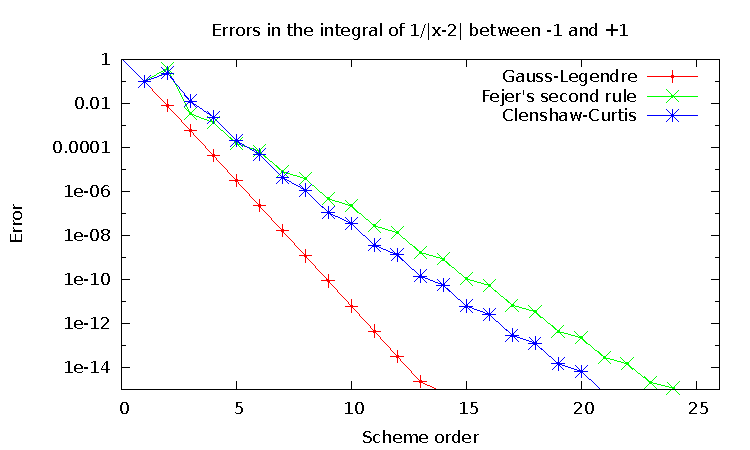
\includegraphics[width=0.75\textwidth]{./quadrature/images/quadrature_errors_xm2}
  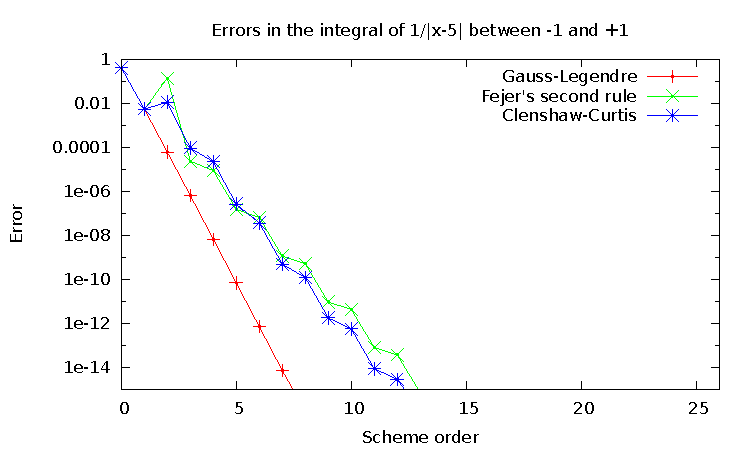
\includegraphics[width=0.75\textwidth]{./quadrature/images/quadrature_errors_xm5}
  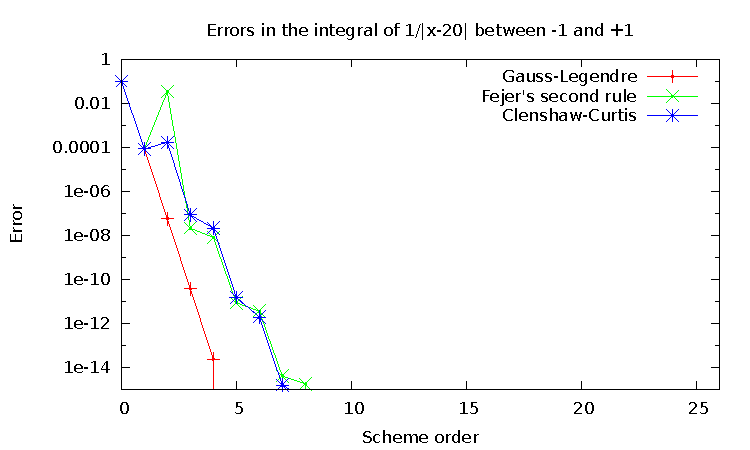
\includegraphics[width=0.75\textwidth]{./quadrature/images/quadrature_errors_xm20}
  \caption{
    \label{fig:exact_quad_errors}
    Comparison of quadrature scheme errors against analytical results in simple near-singular integrals.
  }
\end{figure}



??ds ``predictive'' vs adaptive

??ds storing values between integrations




%%% Local Variables:
%%% mode: latex
%%% TeX-master: "../lit_review_main"
%%% End:



